\documentclass[10pt,pdf,hyperref={unicode}]{beamer}

\mode<presentation>
{
\usetheme{boxes}
\beamertemplatenavigationsymbolsempty

\setbeamertemplate{footline}[page number]
\setbeamersize{text margin left=0.5em, text margin right=0.5em}
}

\usepackage[utf8]{inputenc}
\usepackage[english, russian]{babel}
\usepackage{bm}
\usepackage{multirow}
\usepackage{ragged2e}
\usepackage{indentfirst}
\usepackage{multicol}
\usepackage{subfig}
\usepackage{amsmath,amssymb}
\usepackage{enumerate}
\usepackage{mathtools}
\usepackage{comment}
\usepackage{multicol}

\usepackage[all]{xy}

\usepackage{tikz}
\usetikzlibrary{positioning,arrows}

\tikzstyle{name} = [parameters]
\definecolor{name}{rgb}{0.5,0.5,0.5}

\usepackage{caption}
\captionsetup{skip=0pt,belowskip=0pt}

\newtheorem{rustheorem}{Теорема}
\newtheorem{russtatement}{Утверждение}
\newtheorem{rusdefinition}{Определение}

% colors
\definecolor{darkgreen}{rgb}{0.0, 0.2, 0.13}
\definecolor{darkcyan}{rgb}{0.0, 0.55, 0.55}

\AtBeginEnvironment{figure}{\setcounter{subfigure}{0}}

\captionsetup[subfloat]{labelformat=empty}

%----------------------------------------------------------------------------------------------------------

\title[]{Creating a personalized avatar of a person for a virtual fitting of clothes}
\author{Ksenofontov\,G.\,S.}

\institute[]{Moscow Institute of Physics and Technology (National Research University)}
\date[2022]{\small 14\;december\;2022}

%---------------------------------------------------------------------------------------------------------
\begin{document}

\begin{frame}
\titlepage
\end{frame}

%----------------------------------------------------------------------------------------------------------
\section{Research}
\begin{frame}{Research}
\bigskip
The problem of virtual clothes fitting is investigated.
\begin{block}{Research objective~---}
suggest a method of creation personalized 3D avatar for a virtual fitting of clothes.
\end{block}
\begin{block}{Required to suggest}
\justifying
\begin{enumerate}[1.]
    \item method of generating 3D model parameters,
    \item method of fitting and loose checking of the clothes on 3D avatars.
\end{enumerate}
\end{block}
% \begin{block}{Solution}
% Для \ldots.
% \end{block}
\end{frame}

%---------------------------------------------------------------------------------------------------------
\section{Related papers}
\begin{frame}{Related papers}
\begin{enumerate}[1.]
    \item \textit{Realistic, Animatable Human Reconstructions for Virtual Fit-On}\footnote{\url{https://arxiv.org/pdf/2210.08535.pdf}}: given the main pipeline of online garment fitting
    \item \textit{STAR: A Sparse Trained Articulated Human Body Regressor}\footnote{\url{https://star.is.tue.mpg.de/}}: state-of-the-art and light computational human model
    \item \textit{Keep it SMPL: Automatic Estimation of 3D Human Pose and Shape from a Single Image}\footnote{\url{https://arxiv.org/pdf/1607.08128.pdf}}: generating a 3D human model from image 
    \item \textit{Predicting Loose-Fitting Garment Deformations Using Bone-Driven Motion Networks}\footnote{\url{https://arxiv.org/pdf/2205.01355.pdf}}: generates realistic motion of clothes and predicts the looseness of it. 
\end{enumerate}
% \bigskip
% \footnotetext[1]{\textit{Lopez-Paz D., Bottou L., Scholkopf B., Vapnik V.} Unifying distillation and privileged information // ICLR, 2016.}
% \footnotetext[2]{\textit{Hinton G., Vinyals O., Dean J.} Distilling the knowledge in a neural network // NIPS, 2015.}
\end{frame}

% %---------------------------------------------------------------------------------------------------------
% \section{Problem statement}
% \begin{frame}{Problem statement}
% It is given
% \begin{enumerate}[1.]
%     \item features of body shape,
%     \item image of a person,
%     \item target.
% \end{enumerate}

% \ldots

% \bigskip

% Требуется выбрать модель \ldots из множества
% \[
% 	\mathfrak{G} = \left\{\mathbf{g}| \mathbf{g}:\mathbb{R}^{n} \to \mathbb{Y}^\prime\right\}.
% \]
% Оптимизационная задача \ldots:
% \[
% 	\mathbf{g} = \arg\min_{\mathbf{g} \in \mathfrak{G}} \mathcal{L}\bigr(\ldots\bigr),
% \]
% где $\mathcal{L}$~--- функция ошибки.

% \end{frame}

%---------------------------------------------------------------------------------------------------------
\section{Future work plan}
\begin{frame}{Future work plan}
\begin{enumerate}[1.]
    \item creation of model that generates STAR model parameters,
    \item investigation of clothes problem (dataset and fitting),
    \item investigate the hair problem.
\end{enumerate}
\end{frame}

% %----------------------------------------------------------------------------------------------------------
% \section{Предложенный метод \ldots}
% \begin{frame}{Предложенный метод \ldots}
% ~\\[-1mm]
% Заданы
% \begin{enumerate}[1)]
% 	\item \ldots,
% 	\item \ldots.
% \end{enumerate}

% \medskip
% Параметрические семейства:
% \[
% \setlength\abovedisplayskip{0pt}
% \mathfrak{F} = \left\{\mathbf{f}| \mathbf{f} = \text{softmax}\bigr(\mathbf{v}\bigr(\mathbf{x}\bigr)/T\bigr), \quad \mathbf{v}: \mathbb{R}^{n} \to \mathbb{R}^K \right\},
% \]
% \[
% \mathfrak{G} = \left\{\mathbf{g}| \mathbf{g} = \text{softmax}\bigr(\mathbf{z}\bigr(\mathbf{x}\bigr)/T\bigr), \quad \mathbf{z}: \mathbb{R}^n \to \mathbb{R}^K \right\},
% \]
% где~\ldots.

% \medskip
% Функция ошибки
% \[
% \setlength\abovedisplayskip{0pt}
% \begin{aligned}
%    \mathcal{L}\bigr(\mathbf{g}\bigr) = &-\sum_{i=1}^{m}\underbrace{{\sum_{k=1}^{K}y^k_i\log\mathbf{g}\bigr(\mathbf{x}_i\bigr)\bigr|_{T=1}}}_{\text{исходная функция потерь}}- \sum_{i=1}^{m}\underbrace{{\sum_{k=1}^{K}\mathbf{f}\bigr(\mathbf{x}_i\bigr)\bigr|_{T=T_0}\log\mathbf{g}\bigr(\mathbf{x}_i\bigr)\bigr|_{T=T_0}}}_{\text{слагаемое дистилляции}},
% \end{aligned}
% \setlength\belowdisplayskip{0pt}
% \]
% где~\ldots.

% Оптимальная модель выбирается из класса,
% $\hat{\mathbf{g}} = \arg\min\limits_{\mathbf{g} \in \mathfrak{G}_{\text{cl}}} \mathcal{L}\bigr(\mathbf{g}\bigr).$
% \end{frame}

% %----------------------------------------------------------------------------------------------------------
% \section{Анализ предложенного метода \ldots}
% \begin{frame}{Анализ предложенного метода \ldots}
% \justifying

% На графике показана зависимость значения параметров$w_i$ в зависимости от параметра~$l_1$-регуляризации~$C$.
% \begin{figure}[h!]
% 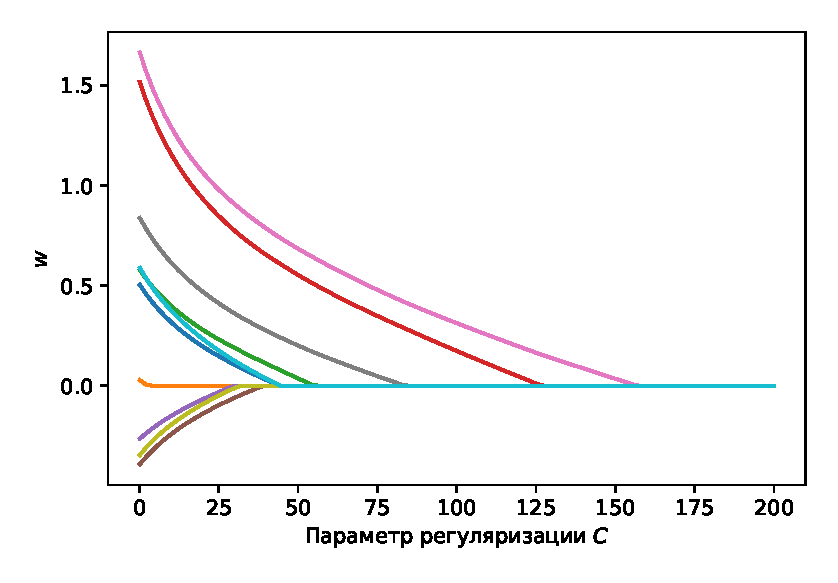
\includegraphics[width=0.45\textwidth]{../figures/log_reg_cs_exp.eps}
% 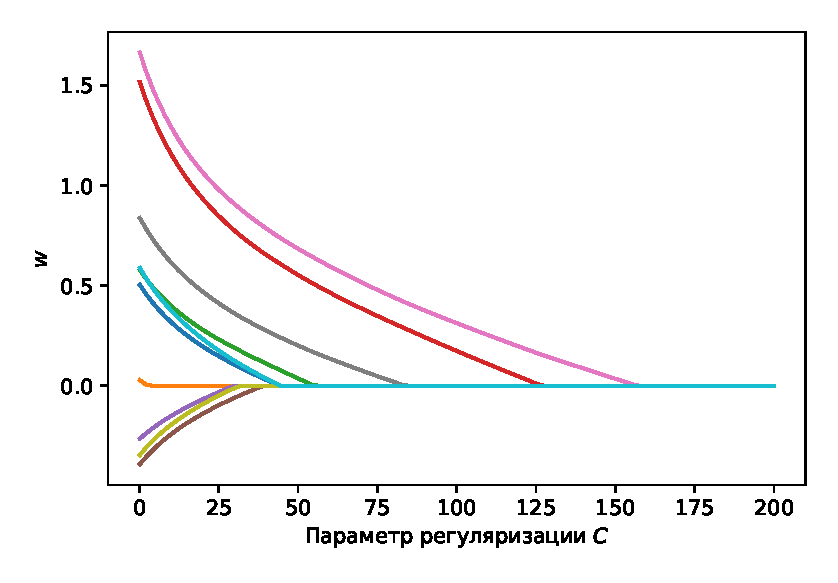
\includegraphics[width=0.45\textwidth]{../figures/log_reg_cs_exp.eps}
% \end{figure}

% С увеличением параметра регуляризации~$C$ число ненулевых параметров~$w_i$ уменьшается.

% \end{frame}

% %----------------------------------------------------------------------------------------------------------
% \section{Выводы}
% \begin{frame}{Выводы}
% \justifying
% 	\begin{enumerate}
% 	\justifying
% 	    \item Предложен \ldots.
%         \item Доказаны теоремы \ldots, 
%         \begin{itemize}
%             \item[---] \ldots,
%             \item[---] \ldots.
%         \end{itemize}
%         \item Предложен метод \ldots
%         \begin{itemize}
%             \item[---] \ldots,
%             \item[---] \ldots.
%         \end{itemize}
%         \item Предложены методы \ldots
%         \begin{itemize}
%             \item[---] \ldots,
%             \item[---] \ldots.
%         \end{itemize}
%         \item Предложена вероятностная интерпретации \ldots.
% 	\end{enumerate}
% \end{frame}
% %----------------------------------------------------------------------------------------------------------

\end{document} 